
\documentclass[12pt]{article}
\usepackage[T1]{fontenc}
\usepackage[utf8]{inputenc}
\usepackage[brazil]{babel}
\usepackage{graphicx}
\usepackage{hyperref}
\usepackage{fancyhdr}
\usepackage{background}
\usepackage[a4paper,top=3.5cm,left=3cm,right=3cm,bottom=2.5cm]{geometry}
\usepackage{lmodern}
\usepackage{tikz}
\usepackage[font={small,stretch=0.80,it}]{caption}
\usepackage{tcolorbox}

%Configurando caixa personalizada
\newtcolorbox{caixa}{colback=red!5!white,colframe=red!75!black}

%Configurando o mapa mental
\usetikzlibrary{mindmap}

%Configurando a path das imagens
\graphicspath{{../../imagens/capitulo5/}}

%Configurando a imagem de background
\backgroundsetup{
scale=1,
angle=0,
opacity=0.4,
contents={%
  
\includegraphics[width=\paperwidth,height=\paperheight]{wallpaper.png}
  }%
}

%configurando os hyperlinks
\hypersetup{
    colorlinks=true,
    linkcolor=green,
    filecolor=magenta,      
    urlcolor=blue,
}

%configurando os headers
\pagestyle{fancy}
\fancyhf{}
\rhead{LDO}
\lhead{Capítulo 5}
\rfoot{Página \thepage}

%configurando identação e separação de parágrafos
\parindent 1.27cm
\parskip   6pt

%títulos,autor e data
\title{\textbf{Capítulo 5 \\ Machine Learning e Embarcados Veiculares}}
\author{Gustavo Lopes Rodrigues}
\date{Novembro de 2020}

\begin{document}
    
    %Inserindo o título
    \maketitle

    \begin{center}
        \begin{tikzpicture}[mindmap, grow cyclic, every node/.style=concept, concept color=orange!40,
        level 1/.append style={level distance=5cm,sibling angle=90},
        level 2/.append style={level distance=3cm,sibling angle=45}]

        \node{Machine Learning e Embarcados Veiculares}
            child [concept color=yellow!30] { node {Embarcados Veiculares \\ \ref{sec:embarcado}}
                child { node {Sistemas compostos}}
                child { node {Micro processadores}}
                child { node {Park Assist}}
            }
            child [concept color=blue!30] { node {A história dos carros\\ \ref{sec:carros}}
                child { node {Motor a vapor}}
                child { node {Motor a eletricidade}}
                child { node {Motor a combustão}}
            };
        \end{tikzpicture}

    \end{center}

    %Configurando uma imagem
    \newpage    

    \begin{caixa}

        \begin{center}

            \href{https://soundcloud.com/gustavo-rodrigues-468052117/ldo-machine-learning-capitulo04}{Ouça o Podcast desse PDF!}
            
        \end{center}

    \end{caixa}

    \section{Inicio} 

        Agora que você acompanhou o Aprendizado de Máquina ao longo de sua evolução, e entende também algumas das características
        sobre o seu funcionamento e inclusive vários exemplos de suas implementações. Neste módulo iremos ver um outro ramo onde 
        Machine Learning tem sido muito utilizado: Embarcados Veiculares

    \section {Um pouco sobre carros} \label{sec:carros}

        Como visto anteriormente, a história do campo do Aprendizados de máquinas é antigo, assim também como também a história 
        dos automóveis, que possuir origens que no século XVIII(18), com a invenção dos carros à vapor. Nós não vamos entrar em 
        detalhe nessa história evolutiva, e por isso, se você quiser ver mais sobre o assunto, deixarei links no final desse PDF, 
        mas em resumo, vamos pontuar os principais pontos da evolução dos carros:

        \begin{itemize}

            \item \textbf{\emph{1769}} - Criação do primeiro motor a vapor, pelo frânces Nicolas-Joseph Cugnot, e que realmente funcionou. Essa primeira geração de carros
            se tornaram prevalentes pelos próximos cem(100) anos, porém se tornou obsoleto, devido a sua pesada caldeira, o que limitiva 
            as atividades que o mesmo podia fazer;

            \begin{figure}[htp]

                \centering
                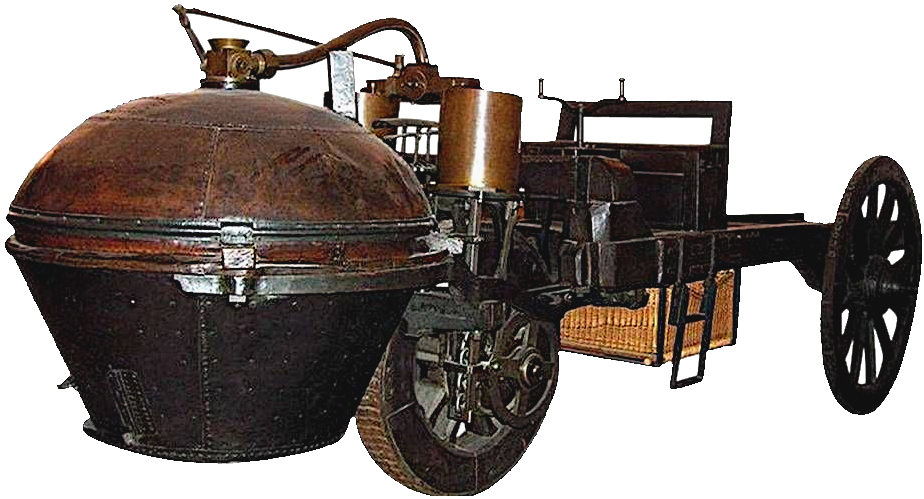
\includegraphics[scale=0.5]{vapor.png}
                \caption{\centering Máquina de Cugnot}

            \end{figure}

            \item \textbf{\emph{1835}} - Construção do primeiro carro elétrico, feito por Thomas Davenport. Infelizmente o uso de carros elétricos 
            não se popularizou, e por conta disso, o uso de veículos elétricos foram adaptados para trilhos.

            \begin{figure}[htp]

                \centering
                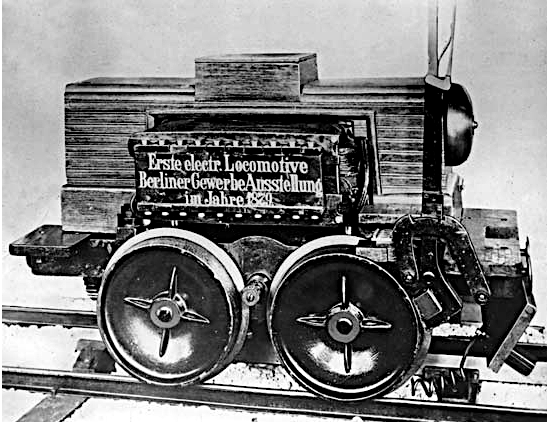
\includegraphics[scale=0.8]{eletrica.png}
                \caption{\centering Locomotiva elétrica}

            \end{figure}

            \newpage

            \item \textbf{\emph{1886}} - Karl Benz registrou o primeiro carro com motor a combustão e com a ajuda de sua esposa, Bertha
            Benz, conseguiram provar que o seu carro tinha funções cotidianas e valia o investimento.

            \begin{figure}[htp]

                \centering
                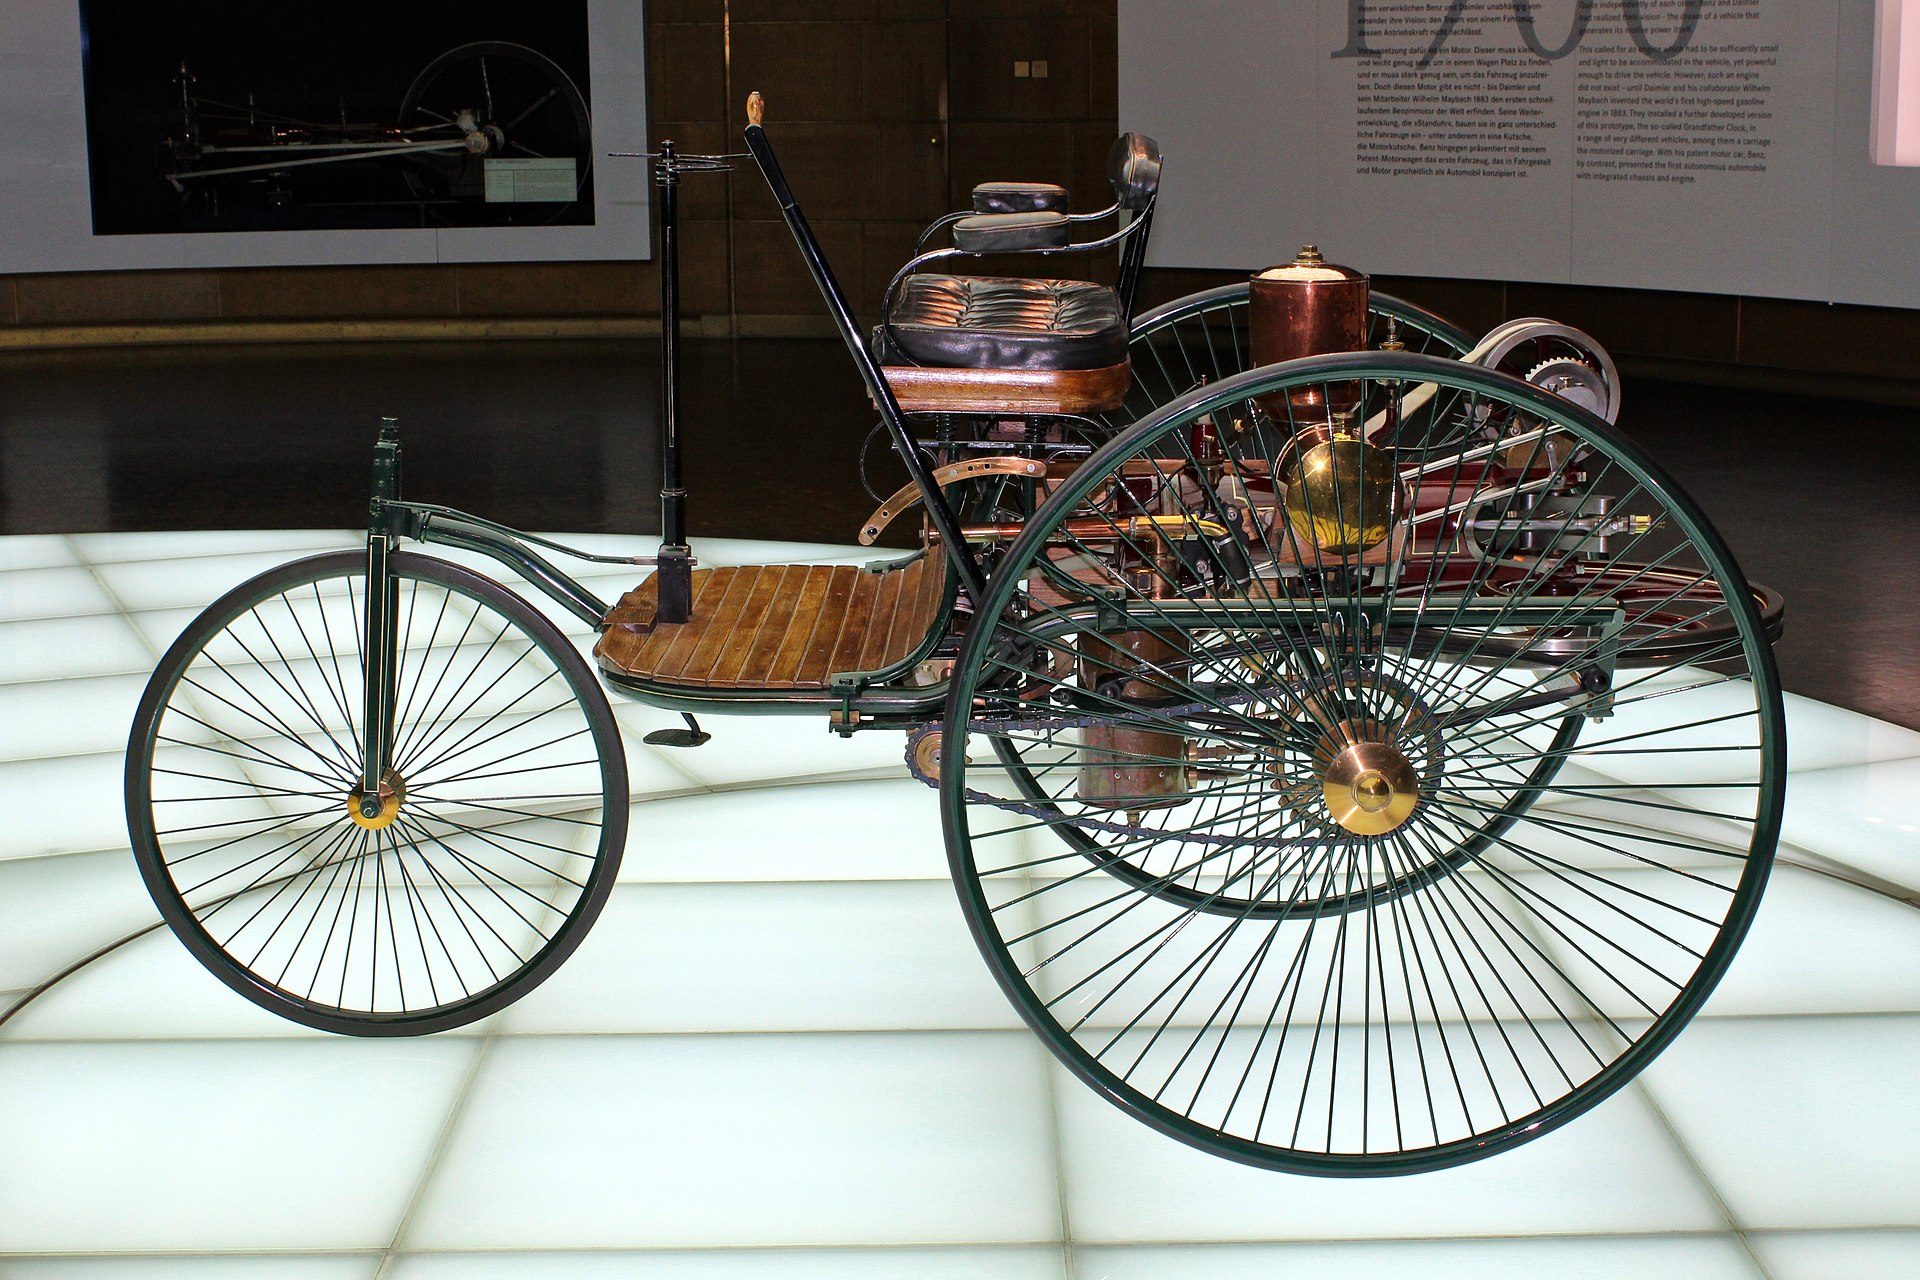
\includegraphics[scale=0.1]{combustao.jpg}
                \caption{\centering Carro com motor a combustão de Karl Benz}

            \end{figure}

            \item \textbf{\emph{1908}} - Lançamento do \emph{Ford Model T} ou como ficou conhecido \emph{Ford Bigode}, que é considerado o primeiro carro popular
            da história.

            \begin{figure}[htp]

                \centering
                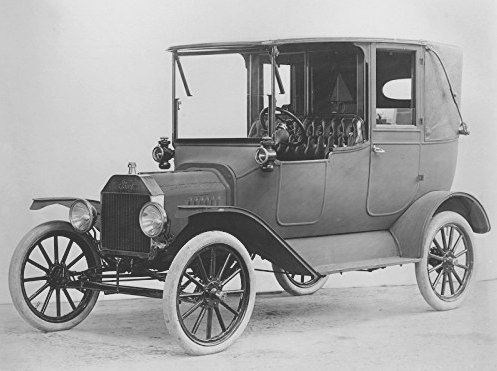
\includegraphics[scale=1]{modelt.png}
                \caption{\centering Foto do carro \emph{Ford Model T}}

            \end{figure}

    \end{itemize}

    \section{Eletrônica Embarcada} \label{sec:embarcado}

    Mas então fica ai a grande pergunta: \textbf{\emph{O que são Embarcados veiculares?}} Bem de acordo com a definição, é a integração dispositivos eletrônicos, como
    microprocessadores e sistemas compostos para ampliar as funcionalidades dos automóveis.

    Alguns exemplos de embarcados veiculares são:

    \begin{itemize}

        \item Computador de bordo 
        
        \item freios ABS
        
        \item airbags 
        
        \item controle de tração
        
        \item ar-condicionado
        
    \end{itemize}

    A partir dos exemplos, é notável que esse conceito já é relativamente antigo, considerando
    que a \href{https://canaltech.com.br/produtos/O-que-e-Computacao-Ubiqua/}{Computação Ubígua} 
    começou a chegar aos automóveis, em torno da década de 70 e 80, com a chegada
    do \emph{freios ABS} e do \emph{Computador de bordo}.

    É claro também que os exemplos citados acima são até bastente conhecidos. O que muitos de vocês
    não devem saber, é sobre as inovações que estão acontecendo na atualidade.

    \section{Park Assist}

    \textbf{\emph{Park Assist}} ou como também é conhecido: Sistema Avançado de Orientação de Estacionamento 
    é uma forma de assistência automatizada de estacionamento, que utiliza-se de radar, câmeras e sensores.
    
    Essa forma de eletrônica embarcada, foi primeiramente introduzida pela Toyota em 1999, para o mercado 
    japônes com o \href{https://en.wikipedia.org/wiki/Toyota_Prius}{Hybrid Prius}. Atualmente, 
    marcas como Volkswagen e Chevrolet, também possuem esse sistema de Park Assist.

    \begin{figure}[htp]

        \centering
        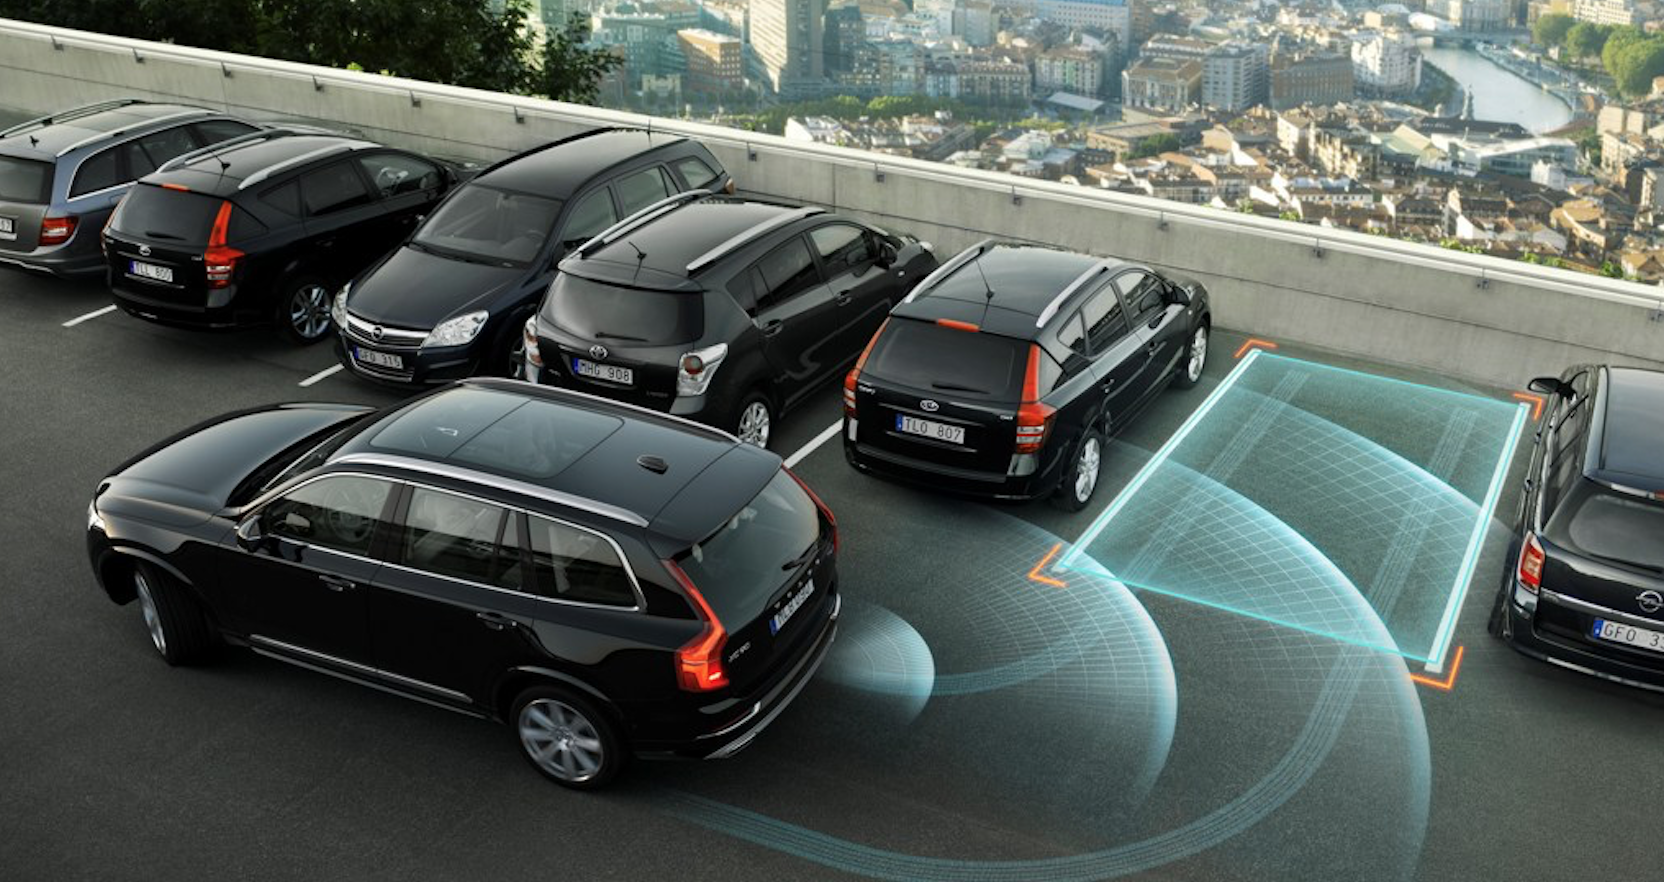
\includegraphics[scale=0.2]{ParkAssist.png}
        \caption{\centering Foto ilustrativa de um carro recebendo auxílio do Park Assist para estacionar}

    \end{figure}

    \newpage 
    
    \section{Conclusão}

    Então, chegamos ao fim desse pequeno módulo sobre Embarcados veiculares, se você se interessou pelo assunto
    ,eu te faço o convite para dar uma leitura ao LDO de Embarcados Veiculares, que você
    pode acessar, a partir \href{https://solid-titans.github.io/LDO-Embarcados-Veiculares/}{desse link}.

    \newpage
    \section*{\centering Material extra}\label{sec:extra} %Criando uma tag para que possa ser referência em outras partes do programa

    %Iniciando listagem
    \begin{itemize}
        
        \item \href{https://www.youtube.com/watch?v=sZVfhWCfz2g}{\textbf{Conheça mais sobre a história dos carros}}
        
        \item \href{https://www.youtube.com/watch?v=XppU8kKpa6I}{\textbf{Veja um vídeo sobre Sistemas Embarcados}}
    
        \item \href{https://www.youtube.com/watch?v=oVBvOwyCFmg}{\textbf{Assista um vídeo do Park Assist funcionando na prática}}

    \end{itemize}

    %Iniciando referências
    \begin{thebibliography}{6}

        \bibitem{eletrico} 
        Veículos elétricos \\
        \href{https://pt.wikipedia.org/wiki/Ve%C3%ADculo_el%C3%A9trico}{\textbf{Um pouco da história dos motores elétricos e os autómoveis}} 
        
        \bibitem{combustão} 
        Veículos à combustão \\
        \href{https://autoesporte.globo.com/carros/noticia/2016/01/130-anos-da-patente-do-primeiro-automovel.ghtml}{\textbf{Sobre o primeiro carro a combustão}}

        \bibitem{vapor} 
        Veículos a vapor \\
        \href{http://www.sinaldetransito.com.br/curiosidades_foto.php?IDcuriosidade=38}{\textbf{A história dos motores a vapor}}
        
        \bibitem{aula} 
        Aula da UNIVESP \\
        \href{https://youtu.be/ElIMxXcFkGQ}{\textbf{Aula introdutória a Eletrônica Embarcada}}

        \bibitem{bordo} 
        Computadores de bordo \\
        \href{https://loucosporcarro.com.br/computadores-de-bordo/}{\textbf{A história dos computadores de bordo no Brasil}}

        \bibitem{parkassist} 
        Park Assist \\
        \href{https://en.wikipedia.org/wiki/Intelligent_Parking_Assist_System}{\textbf{Referência}}
    \end{thebibliography}

    

\end{document}